
\section{Bayesian thinking}

\begin{frame}{Intended Learning Outcomes}

        At the end of this day you will be able to:
        \begin{itemize}
                \item appreciate the use of Bayesian statistics in life sciences,
                \item formulate and explain Bayes' theorem.
		\item describe a Normal-Normal model and implement it in \texttt{R} with
		or without Monte Carlo sampling,
                \item apply Bayesian statistics to estimate genotypes from DNA sequencing data.
        \end{itemize}

\end{frame}

\begin{frame}{Meet Nessie}

	\begin{figure}[!ht]
		\centering
		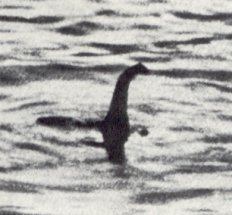
\includegraphics[width=4cm]{Images/LochNessMonster.jpg}
		\caption{Nessie, the Loch Ness Monster. True or fake news?}
		\label{Fig:LochNess}
	\end{figure}

\end{frame}

\begin{frame}{Likelihood for a monster to exist (!?)}

	\begin{itemize}
		\item $D = \{0,1\}$ be our data, whether I tell you I saw Nessie or not.
		\item $\theta = \{0,1\}$ is the probability distribution for Nessie existing (or not).
	\end{itemize}

	\begin{block}{Questions}
		\begin{itemize}
			\item What are $p(D=1|\theta=1)$ and $p(D=1|\theta=0)$?
			\item What is a Maximum Likelihood Estimate of $N$?
		\end{itemize}
	\end{block}

\end{frame}

\begin{frame}{Likelihood thinking...}

	Our inference on $\theta$ is driven solely by our observations, given by our likelihood function.

	\begin{figure}[!ht]
		\centering
		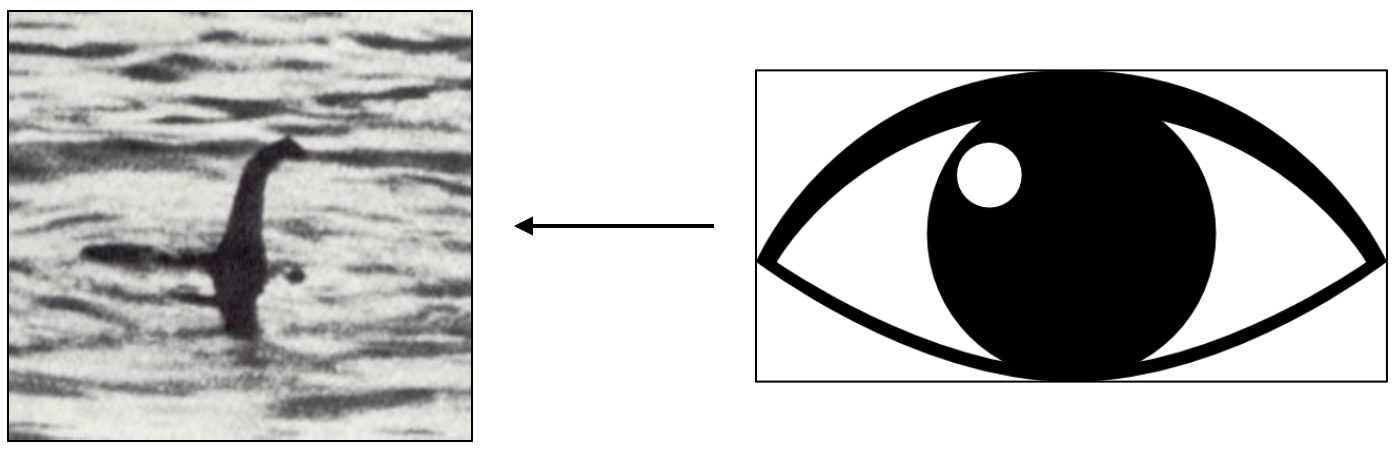
\includegraphics[width=5cm]{Images/EyeOnly.png}
		\caption{The eye: a "likelihood" organ.}
		\label{Fig:EyeOnly}
	\end{figure}

\end{frame}

\begin{frame}{Non-likelihood thinking...}

	In real life we take many decisions based not only on what we observe but also on some believes of ours.

	\begin{figure}[!ht]
		\centering
		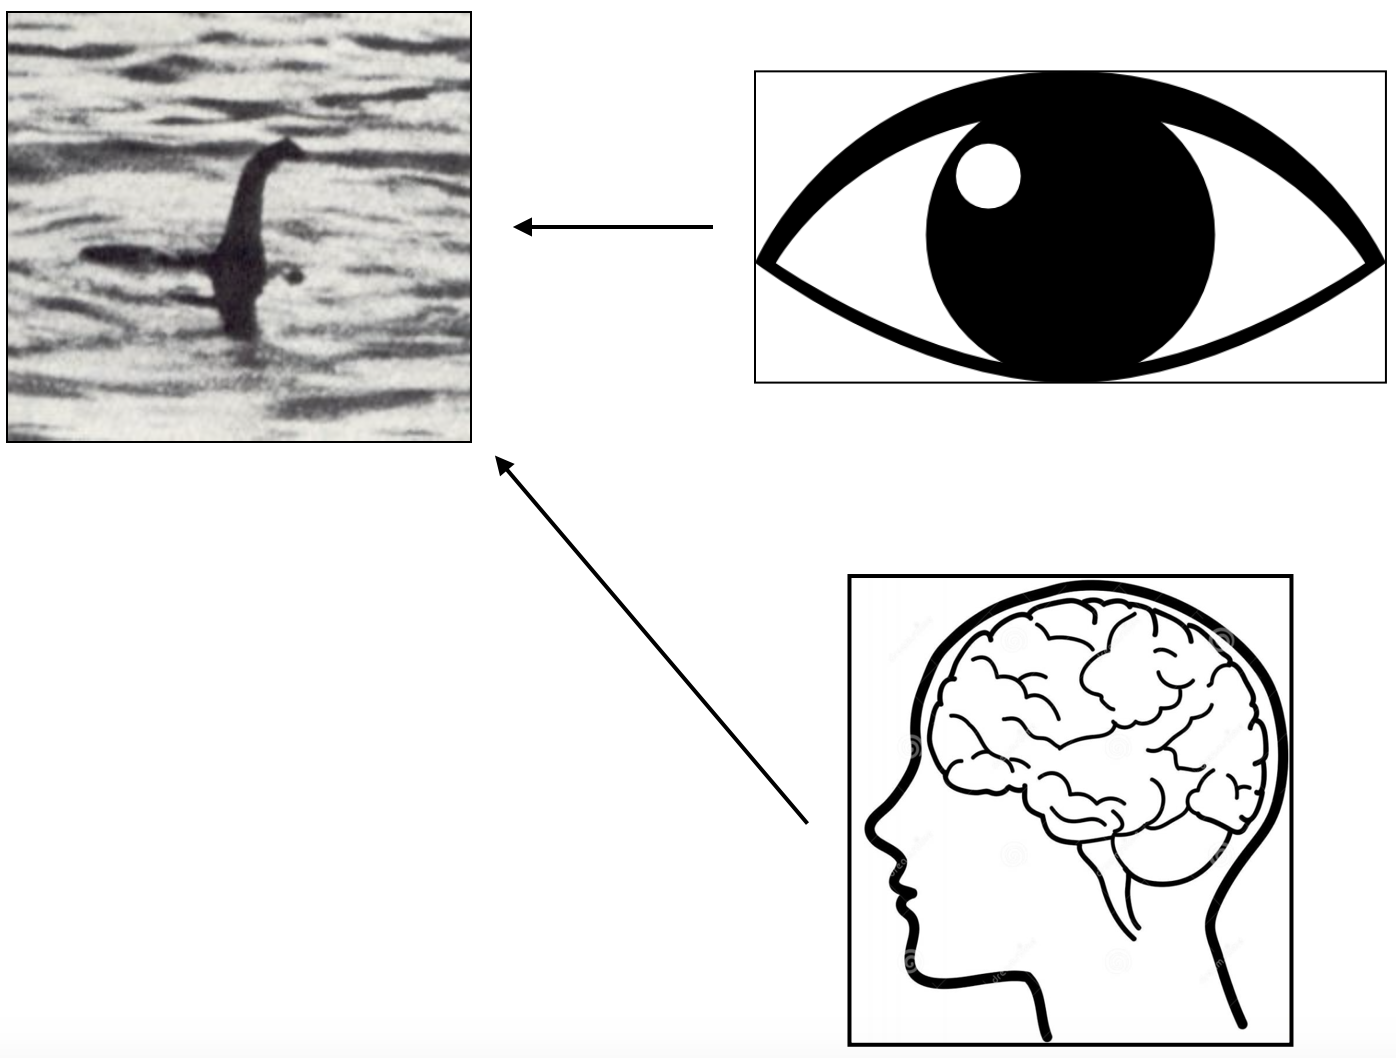
\includegraphics[width=5cm]{Images/EyeBrain.png}
		\caption{The brain: a "non-likelihood" organ.}
		\label{Fig:EyeBrain}
	\end{figure}

\end{frame}

\begin{frame}{Bayesian thinking}

	\begin{itemize}
		\item with "eyes only" our intuition is that $p(\theta|D) \propto p(D|\theta)$
		\item with "the brain" our intuition is that $p(\theta|D) \propto p(D|\theta)p(\theta)$
	\end{itemize}

	Our "belief" expresses the probability $p(\theta)$ \textbf{unconditional} of the data.

	\begin{block}{Question}
		How can we define $p(\theta)$?
	\end{block}

\end{frame}

\begin{frame}{Prior and posterior probability}

	\begin{block}{}
		The "belief" function $p(\theta)$ is called \textbf{prior probability} and the 
		joint product of the likelihood $p(D|\theta)$ and the prior is proportional 
		to the \textbf{posterior probability} $p(\theta|D)$.
	\end{block}

	\begin{block}{}
		The use of posterior probabilities for inferences is called Bayesian statistics.
	\end{block}

\end{frame}

\begin{frame}{Bayesian statistics}

	Bayesian statistics is an alternative to frequentist approaches but without a definite division as in many cases 
	the approach taken is \textbf{eclectic}.

	\begin{figure}[!ht]
		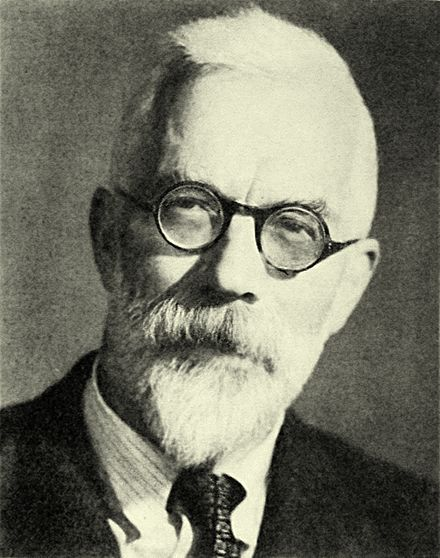
\includegraphics[width=2cm]{Images/Ronald_Fisher.jpg}
		\caption{Ronald Fisher.}
	\end{figure}

\end{frame}

\begin{frame}{Publishing a paper}

	Example:\\
	You submitted a manuscript for publication to a peer-reviewed journal and you want to assess its probability 
	of being accepted and published.

	\begin{figure}[!ht]
         	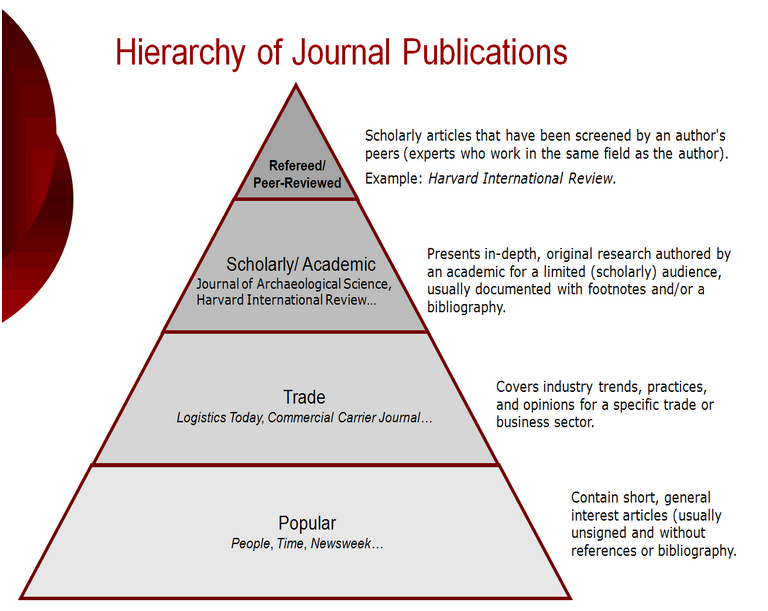
\includegraphics[width=3.5cm]{Images/journals.png}
        \end{figure}

	Which information do you need (and use) to make such inference?

\end{frame}

\begin{frame}{Measuring biodiversity}

	Example:\\
	You are measuring the biodiversity of crabs on Scottish rock shores in four different 
	locations over three years.

	\begin{table}
		\centering
		\caption{Biodiversity levels.}
		\begin{tabular}{c|cccc}
			Year & Loc. A & Loc. B & Loc. C & Loc. D\\
			2016 & 45 & 54 & 47 & 52\\
			2017 & 41 & ? & 43 & 45\\
			2018 & 32 & 38 & 37 & 35\\
		\end{tabular}
	\end{table}

	\begin{block}{Question}
		What is a reasonable value for the missing entry?
	\end{block}

\end{frame}

\begin{frame}{Statistical inference}

	\begin{itemize}
		\item Frequentist (from data only)
		\item Likelihoodist (using a statistical model)
		\item Bayesian (using prior information)
		\item Empirical Bayesian (observed data contribute to the prior)
	\end{itemize}

	\begin{figure}[!ht]
		\centering
		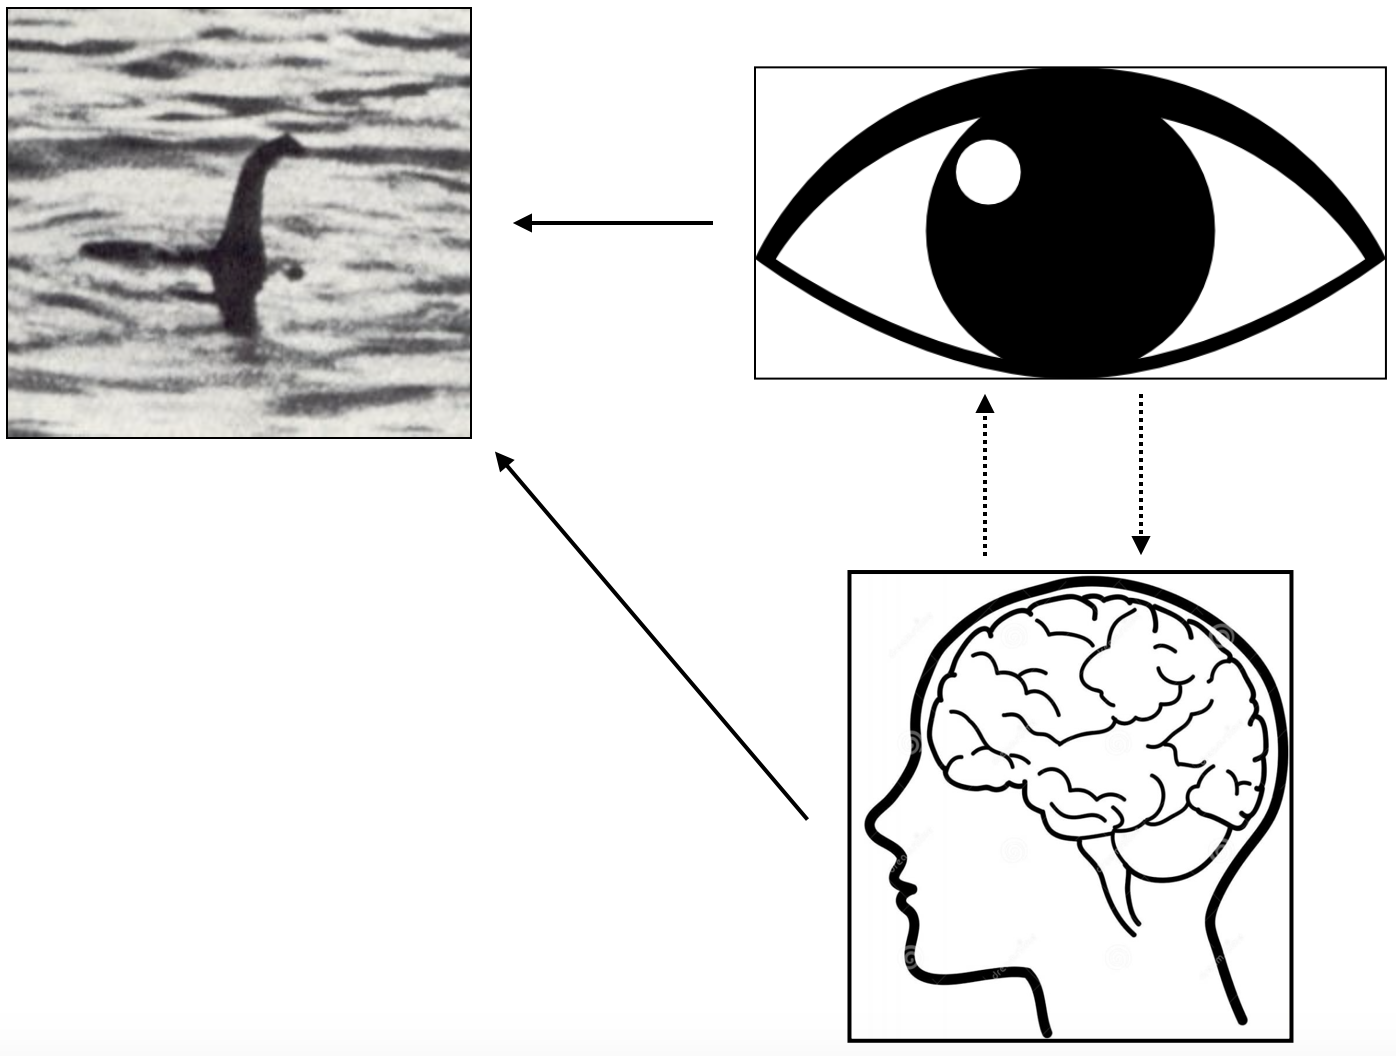
\includegraphics[width=3cm]{Images/EyeBrainEB.png}
		\caption{The brain \textbf{and} the eye: an Empirical Bayesian organ.}
		\label{Fig:EyeBrainEB}
	\end{figure}

\end{frame}

\begin{frame}{Statistical inference}

	If $D$ is the data and $\theta$ is your unknown parameter, then
	\begin{itemize}
		\item the frequentist conditions on parameters and integrates over the data, $p(D|\theta)$,
		\item the Bayesian conditions on the data and integrates over the parameters, $p(\theta|D)$.
	\end{itemize}

\end{frame}

\begin{frame}{Bayesian \textit{vs.} Likelihoodist:}

	\begin{itemize}
		\item we derive "proper" probability distributions of our parameters 
		rather than deriving a point estimate,
		\item a probability is assigned to a hypothesis rather than a hypothesis is tested,
		\item we "accept" the null hypothesis rather than "fail to reject" it,
		\item parsimony imposed in model choice rather than correcting for multiple tests.
	\end{itemize}

\end{frame}

\begin{frame}{History}

	\begin{columns}
		\column{0.5\textwidth}
		\begin{figure}
			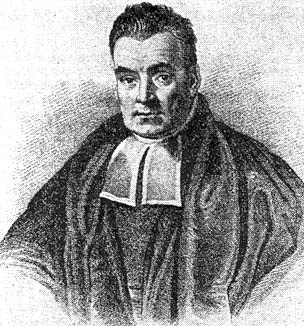
\includegraphics[width=2cm]{Images/ThomasBayes.jpeg}
			\caption{Rev. Thomas Bayes}
		\end{figure}
		\column{0.5\textwidth}
		\begin{figure}
			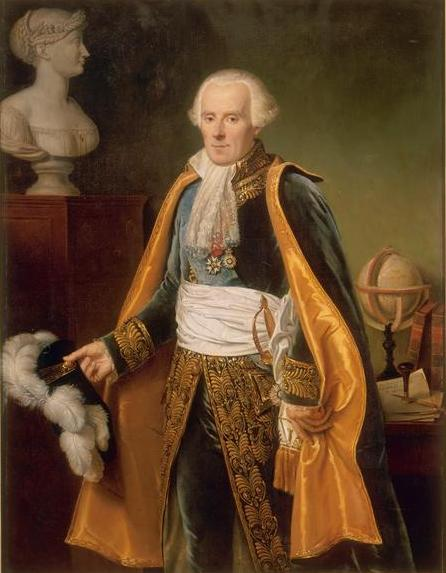
\includegraphics[width=2cm]{Images/Laplace.jpg}
			\caption{Pierre-Simon, marquis de Laplace}
		\end{figure}
	\end{columns}

\end{frame}

\begin{frame}{Why?}

	\begin{block}{Why is Bayesian statistics becoming so commonly used?}
		\begin{itemize}
			\item recent increased computing power
			\item good frequentist properties
			\item answers are easily interpretable by non-specialists
			\item already implemented in packages
		\end{itemize}
	\end{block}

\end{frame}

\begin{frame}{Troubles with the \textit{p}-value?}

	\begin{block}{John K. Kruschke (2010)}
		...the fundamental fatal flaw of \textit{p}-values is that 
		they are ill defined, because any set of data has many different \textit{p}-values.

            	...many people mistake the \textit{p}-value for the probability that the null 
		hypothesis is true. 

	\end{block}

\end{frame}

\begin{frame}{Troubles with the prior?}

	\begin{block}{John K. Kruschke (2010)}
		Some people may have the mistaken impression that the advantages of 
		Bayesian methods are negated by the need to specify a prior distribution.
		\begin{itemize}
			\item It is inappropriate not to use a prior.
			\item Priors are explicitly specified and must be agreeable to a skeptical 
			scientific audience.
			\item When different groups of scientists have differing priors, 
			stemming from differing theories and empirical, then Bayesian methods provide 
			rational means for comparing the conclusions from the different priors.
		\end{itemize}
	\end{block}

\end{frame}

\begin{frame}{Why are WE using it?}

	\begin{block}{}
		Bayesian statistics is very used in many topics in life sciences:
		\begin{itemize}
			\item genetics (e.g. fine mapping of disease-susceptibility genes)
			\item ecology (e.g. agent-based models)
			\item evolution (e.g. inference of phylogenetic trees)
			\item bioinformatics (e.g. genome assembly)
			\item systems biology (e.g. gene networks)
			\item ...
		\end{itemize}
		and provides a rationale for other approaches (e.g. artificial neural networks).
	\end{block}

\end{frame}

